\documentclass[11pt, a4paper]{article} 

% Packages
\usepackage[fleqn]{amsmath} % fleqn: flush left equations <-- Left-flush equations
\usepackage{graphicx}

% Format
\usepackage[margin=2cm, top=2cm]{geometry}

% Heading
\title{\bf Design 1\\[1ex]
\rm\normalsize CS202 Programming Systems, Summer 2020 }
\date{\normalsize Due: July, 2, 2020}
\author{\normalsize Armant Touche}

\begin{document}

\vspace{0cm}\maketitle 

\section*{UML Diagram:}


            \begin{center}
            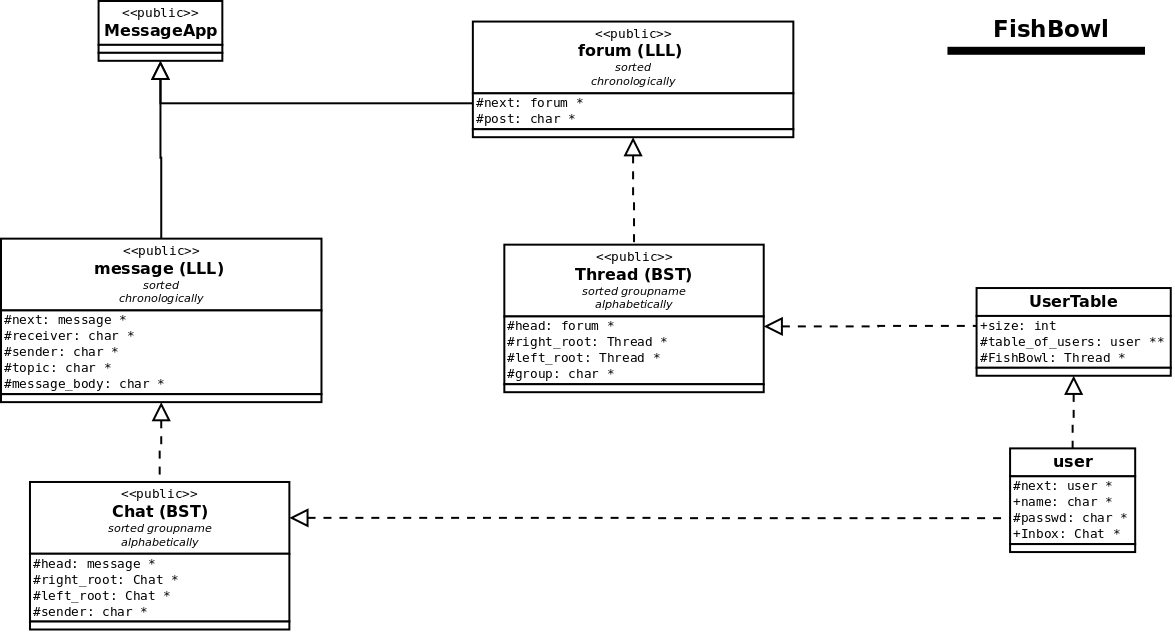
\includegraphics[width=.8\textwidth]{uml3}
            \end{center}

\section*{Write-up:}
This assignment requires us to create a chat application called the "fish bowl" where each user will a inbox that will contain messages from a user. The messages will be chronologically ordered from most recent at the beginning to oldest. The user's inbox will be stored into a binary search tree which will be alphabetically sorted where each sender will contain the linear linked list of messages. For the operator overloading, I will have a string class that act a my base class. I will derive user, sender, and messages from string because each of the derived classes will contain character array variables and I will be overloading the extraction, insertion, subscript, addition, assignment, equality, and prefix operators. This will allow the client program to easy do input and output operations with ease and for classes managing the data structures, the equality operator and subscript operator will come in handy when dealing traversals and/or accessing the user from the table of users.\\
\indent To get started on the program I will first start with the user classes and to make sure that I can create and store users into the table and then finally access each user according to their name and password. Kind of like a login where each user will possess a unique password. Once the client is able to create a user and login to the existing user's account, then separately, I start with the inbox class ensuring that user-class's send-message function creates a sender node within the inbox (binary search tree). But before creating the inbox-class, I will on the string-class which user-node, sender, and message will be derived from the string-class. Again, the reason will be because each derived class will contain character array variables like name, message topic, and message body. Once I am to store users into the binary search tree, I will move on to creating the message-node class next. For each message created, I store them in chronological starting the most recent. Insertion will take place at the head of the linear linked list of messages. I will also keep track of number of messages because I would like to overload the subscript operator. Reason for wanting to overload the subscript operator is because I would like to abstract the traversal with subscript operator allowing for pseudo-instant access but really, I just abstracted the traversal. But, I may run into trouble because I have never implemented anything as such before. I will definitely be attending the homework recitation hours to get feedback from the lab assistants. \\
\indent I will be scouring over the handwritten notes and lecture slides because I am still little unsure on the residual-value and lvalue concepts. The main hurdle for this program will be using dynamic binding in conjunction with operator overloading because again, I am still confused on which operators are required to member functions and which can be friend functions. I think the equality operators can be either member function or not a member function. I think the lvalue is just an integer so I could just prototype my overloaded equality operators as a member or a non-member function. Since I want to dynamic binding within my hierarchy and also, each class will have different implementations because of different data members, I implement as a abstract base class where all of my overloaded equality operators will be pure virtual functions. When I start programming program number three, I will learn some of the nuances that come with operator overloading but right now, I am still a little hesitant on describing my object oriented design. I will be using GNU debugger at each step of the way and think GDB will be my main guide into this program.


\end{document}
